\chapter{Introduction to Programming in OPUS}

This chapter provides a gentle introduction to programming in OPUS.  It is intended not for software developers but for model users, who need to understand enough about the underlying software to be able to use all of the capabilities of the system, and to extend these capabilities.  OPUS is implemented in the Python programming language, so we begin with a review of the language in Section \ref{sec:python}.  Numpy is a numerical library for Python that is used exensively in the OPUS system, so this is covered in Section \ref{sec:numpy}. Using Python and Numpy, many of the OPUS Variables are coded as modules, and these are explained in Section \ref{sec:variables}.  Finally, a recent and extremely valuable addition to the OPUS architecture is a small language for OPUS Expressions, which makes the need to code variables as separate modules unnecessary in most cases.  The expression language is the subject of Section \ref{sec:expressions}.

\section{Python}
\label{sec:python}

Python is a programming language developed initially by Guido van Rossum, and has become a very popular programming language with a large user and developer base.  It has been adopted, for example, by ESRI as the main scripting language for ArcGIS. It is Open Source software, and is available from www.python.org.  Python is an interpreted language, as compared to a compiled language.  This means that when you start Python, you are launching the Python interpreter, which then interacts with commands typed in interactively, or with programs (scripts) loaded from disk. 

Python can be launched in several ways:

\squishlist
\item from the command shell by typing \verb#python#, or from the start menu in Windows
\item from IDLE, a light-weight Python Editor and Shell that comes with Python, which can be launched from the start menu
\item using Scite, an editor that can also run Python programs
\item using a sophisticated Integrated Development Environment (IDE) sush as Eclipse, Wing, or Eric
\squishend

To get started, launch IDLE from the Windows \verb#Start# menu.  It will launch a window as shown in Figure \ref{fig:python-idle}.  If you are not on a Windows computer, just start a command shell and type \verb#python# to start an interactive Python session.

\begin{figure}[htp]
\begin{center}
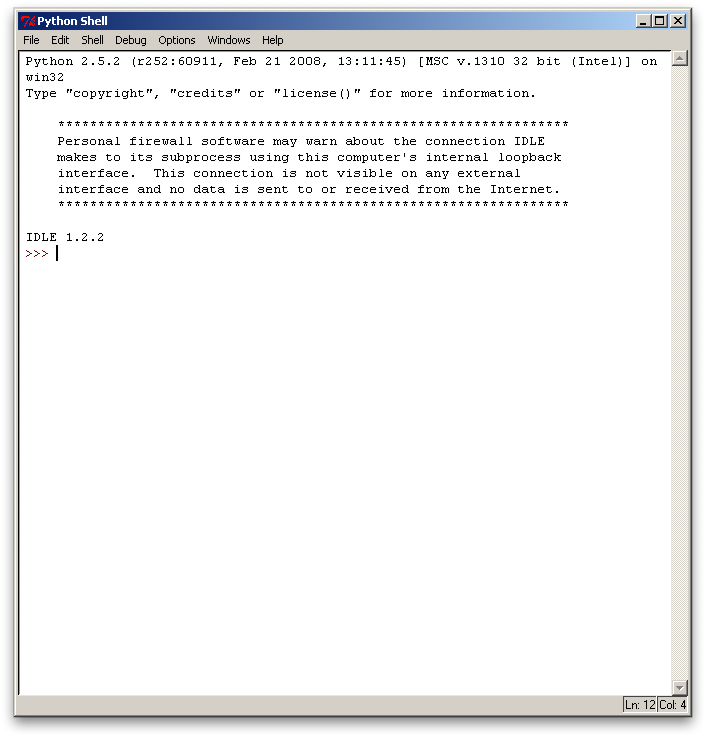
\includegraphics[scale=0.4]{graphics/python-idle.png}
\end{center}
\caption{The IDLE Python Shell}
\label{fig:python-idle}
\end{figure}

\subsection{Expressions and Data Types}

Python has several data types that are useful to understand as you begin to explore the language.  These data types are:

\squishlist
\item integers
\item floats
\item booleans
\item strings
\item tuples
\item lists
\item dictionaries
\squishend

Begin with the basics.  Python can do simple (or complex) calculations interactively, just as you might do with a calculator.  How might you compute the sum of two numbers?  Just type in a mathematical expression, and hit return.  Try 2+2, and 3/2.  Notice that the second answer is probably not what you want: the result is an integer, rather than a floating point, so it truncates.  To get a floating point result, use a decimal place on at least one of the inputs.\\

\begin{lstlisting}
>>> 2+2
4
>>> 3/2
1
>>> 3/2.0
1.5
\end{lstlisting}

The results of expressions are easily assigned to a variable name, and used in further calculations.  Notice that when you type an assignment of an expression to a variable, it does not print the value, but does assign it.  You can print or use the value at this point.  \\

\begin{lstlisting}
>>> a = 2+2
>>> a
4
>>> b = 3/2.0
>>> a+b
5.5
>>> (a+b)/2
2.75
\end{lstlisting}

Now examine what happens if we use operators that \verb#assert# a statement that can be evaluated as \verb#True# or \verb#False#.  This generates a \verb#Boolean# data type.

\begin{lstlisting}
>>> a = 2
>>> b = 4/2
>>> a == b    #This asserts that a is equal to b, by using == instead of =
True
>>> a < b      #This asserts that a is less than b
False
\end{lstlisting}

We have seen so far three of Python's data types: integers, floats, and booleans.  Text is also managed in Python, using its string datatype.  Strings can be assigned to variables, and used, for example to concatenate two strings, or to extract a portion of a string using the index.  Note that Python uses index values starting from 0.  If a single index value is used, then it identifies a single value in the string at the index position.  If two values are used, the second identifies the ending index value.  One behavior that is not intuitive is that the returned values are up to, but do not include the second index value.\\

\begin{lstlisting}
>>> a = 'Conca'
>>> b = 'tenate'
>>> c = a+b
>>> c
'Concatenate'
>>> c[0]
'C'
>>> c[0:2]
'Co'
>>> c[2:]
'ncatenate'
\end{lstlisting}

There are three other data types in Python that are closely related: tuples, lists and dictionaries.  Tuples contain a set of items that are indexed (like strings, above), but cannot be changed once defined.  An example would be the days of the week, or the months of the year:

\begin{lstlisting}
>>> days = ('Monday', 'Tuesday', 'Wednesday', 'Thursday', 'Friday', 'Saturday', 'Sunday')
>>> days[3]
'Thursday'
\end{lstlisting}

Lists are almost the same as tuples, but they can easily be modified, and items can be added or removed. A To Do list would be an example:

\begin{lstlisting}
>>> todo = ['get groceries', 'do homework', 'paint wall', 'watch movie']
>>> todo[1]
'do homework'
>>> todo.append('read book')
>>> todo
['get groceries', 'do homework', 'paint wall', 'watch movie', 'read book']
>>> del todo[1]
>>>todo
['get groceries', 'paint wall', 'watch movie', 'read book']
\end{lstlisting}

Dictionaries are flexible data structures that store key:value pairs, like a standard dictionary stores words and their associated definitions.  Entries can be looked up by their key.  A phonebook provides a simple example.  Note the syntax to add an entry.  Also, pay attention to the use of different kinds of brackets for these different data types.  They do matter, and will generate an error if the wrong one is used.

\begin{lstlisting}
>>> myPhoneBook = {'Mark':2439503, 'Julie':4309302, \
... 'Jeff':3540693}
>>> myPhoneBook['Jeff']
3540693
>>> myPhoneBook['Mary'] = 3339999
>>> myPhoneBook
{'Julie': 4309302, 'Jeff': 3540934, 'Mary': 3339999, 'Mark': 2439503}
\end{lstlisting}

\subsection{Python Modules, Packages, and Methods}

Python commands can be used interactively, as we have just seen,  but they can also be stored in a file, called a Python Module, provided that it ends with an extension of \verb#.py#, and follows some basic formatting requirements, like the use of indentation to identify what statements belong in a block.  More on this later.

Any Python statements you can execute interactively can be put into a Python module and then executed at the command line or loaded into IDLE or another program that can ediot and execute Python modules (Scite is a good example).  Say you have created the classic first program "Hello World" in a Python module, called hello.py.  It would contain one line: \verb#print "Hello World"#, and would be executed by typing at the command shell prompt (not the Python prompt):

\begin{lstlisting}
c:\> python hello.py
Hello World
\end{lstlisting}

Python contains many built-in methods, and we will explore some of them as needed.  One of the most common and useful ones is the range method.  It generates a list, with N entries in it, sequentially numbered, starting from 0.  N is passed to the method as an \verb#argument#, in parentheses, like this:

\begin{lstlisting}
>>> range(10)
[0, 1, 2, 3, 4, 5, 6, 7, 8, 9]
\end{lstlisting}

This is useful in programs in which you need to iterate over a list, or perform some function N times.  Here is the first example in which formatting in Python is needed.  We have to indent the line \verb#print i# underneath the line \verb#for in in range(10):# in order to make clear to the Python interpreter which lines of the script are to be repeated 10 times.  If we put this into a loop.py module and want to print the word "Done!" at the end of the list, the script would look like this:

\begin{lstlisting}
for i in range(10):
	print i
print 'Done!'
\end{lstlisting}

If we have saved this as loop.py, then we can run it at the command prompt by typing \verb#python loop.py#, and would see the following output:

\begin{lstlisting}
0
1
2
3
4
5
6
7
8
9
Done!
\end{lstlisting}



Now that we have used a built-in Python function, try writing one of your own.  For example, you could compute the square of a number with a function like this:

\begin{lstlisting}
def square(n):
	return n*n

print square(111)
\end{lstlisting}

It would not be necessary to implement this particular method, however, since it is built into Python's Math package.  To use functions in the Math package, you have to import the functions or the whole package.  Here are some options:

\begin{lstlisting}
>>> import math
>>> math.sqrt(9)
3
>>> from math import sqrt
>>> sqrt(9)
3
>>> from math import *
>>> log(9)
2.1972245773362196
\end{lstlisting}

Note the difference in usage depending on which way you choose to import a function.  The last one, using a * to import all the functions, is acceptable for an interactive session, but is a poor choice in a complex program you write, because each imported function has a name that gets stored in a Python \verb#Namespace# used to keep track of all the functions, and this can get cluttered or confusing if you happen to import from multiple packages and don't realize that the same function name is used to do different things in two different packages. You will see imports of many packages in the OPUS system.  One of the main ones is covered in the next section: Numpy.


\section{Numpy}
\label{sec:numpy}

Numpy is a Python package (library) for processing multi-dimensional arrays.  To set terminology, consider a spreadsheet in Excel or some similar package.  A data value in a single cell would be a \verb#scalar#, or a single-dimension \verb#array# of length 1.  A column of 10 numbers would be a single-dimensional array of length 10.  A sheet of 10 columns by 15 rows would be a two-dimensional array of shape (10, 15).  If we then use 5 separate worksheets with each one containing a 10 by 15 worksheet, we have a three-dimensional array of shape (10, 15, 5).  Numpy is designed to create, manipulate, and efficiently compute on these arrays.

Let's begin a tour of Numpy by importing it and creating a small array,  and then finding its size and shape, and computing some built-in Numpy functions on it. Note that we can easily manipulate the shape of an array.

\begin{lstlisting}
>>> from numpy import *
>>> a = arange(10)
>>> a
array([0, 1, 2, 3, 4, 5, 6, 7, 8, 9])
>>> a.size
10
>>> a.shape
(10,)
>>> a.sum()
45
>>> a.mean()
4.5
>>> a.std()
2.8722813232690143
>>> a*2
array([ 0,  2,  4,  6,  8, 10, 12, 14, 16, 18])
>>> a.reshape(5,2)
array([[0, 1],
       [2, 3],
       [4, 5],
       [6, 7],
       [8, 9]])
\end{lstlisting}

There are numerous ways to create arrays, including some built-in functions for frequently used arrays containing 0's or 1's, or loading data from a file or even a database (with a bit more work).

\begin{lstlisting}
>>> z = zeros( (3,4) )
>>> z
array([[ 0.,  0.,  0.,  0.],
       [ 0.,  0.,  0.,  0.],
       [ 0.,  0.,  0.,  0.]])
>>> a = array( [2,3,4] )
>>> a
array( [2,3,4] )
\end{lstlisting}

Notice that you can perform mathematical operations on arrays, and that the default is to compute results \verb#elementwise#, or element by element, like you would do in a spreadsheet.  You can also use matrix computations as in linear algebra, with a slightly different syntax.   A matrix multiplication of arrays A and B would be: \verb#dot(A,B)#.  In the examples below, note the use of assignment to a variable (using an =), as compared to the use of an assertion that two arrays are equal (using ==). Also note the use of a where statement, which allows assignment of different values where the statement is evaluated as truo or false.  These examples cover some of the more commonly used manipulations of arrays in OPUS and UrbanSim.

\begin{lstlisting}
>>> a = array( [20,30,40,50] )
>>> b = arange( 4 )
>>> c = a-b
>>> c
array([20, 29, 38, 47])
>>> b**2
array([0, 1, 4, 9])
>>> 10*sin(a)
array([ 9.12945251, -9.88031624,  7.4511316 , -2.62374854])
>>> a<35
array([True, True, False, False], dtype=bool)
>>> where(a<35, 1, 0)
array([1,1,0,0)]
>>> d = array([10,30,20,50)]
>>> a == d
array([False, True, False, True], dtype=bool)
\end{lstlisting}

Numpy provides sophisticated numerical capabilities for doing statistical or econometric modeling, with a very consice syntax.  An example of a tutorial script to estimate  the parameters of a multiple linear regression, using Ordinary Least Squares estimation, is shown in the Appendix to this chapter.  The script is from http://www.scipy.org/Cookbook/OLS.



Numpy contains a very large number of built-in functions. The following, for example, are some built-in random number functions:

\squishlist
\item beta(), binomial(), gumbel(), poisson(), standard\_normal(), uniform(), vonmises(), weibull()
\item rand(), randint(), randn()
\item random\_integers()
\item random\_sample()
\item ranf()
\item sample()
\item seed()
\squishend

For a more complete tutorial on Numpy, please refer to the one at http://www.scipy.org/Tentative\_NumPy\_Tutorial.

\section{OPUS Variables}
\label{sec:variables}

Variables in OPUS are Python modules containing a single Python \verb#Class# that computes a variable and returns the result.  For demonstration purposes, the population variable in \verb#/src/urbansim/gridcell/population.py# is shown below.  We refer to a variable using a \verb#Pythonpath#, which provides a means for Python to find modules and classes in a directory structure.  So, a reference to this particular module using a \verb#fully qualified path# would be \verb#urbansim.gridcell.population#.  You can find all of the existing variables by browsing on disk in the source code directory.  The directory structure mirrors the parts of the variable name, so that urbansim.gridcell.population is really pointing to /opus/src/urbansim/gridcell/population.py, which is included below as an example.

\begin{lstlisting}
from opus_core.variables.variable import Variable
from urbansim.functions import attribute_label
from variable_functions import my_attribute_label
from opus_core.logger import logger

class population(Variable):
    """Compute the total number of people residing in a gridcell, 
    by summing hh_persons over all households in the gridcell"""
    
    _return_type="int32"
    hh_persons = "persons"

    def dependencies(self):
        return [attribute_label("household", self.hh_persons), 
                attribute_label("household", "grid_id"), 
                my_attribute_label("grid_id")]

    def compute(self, dataset_pool):
        households = dataset_pool.get_dataset('household')
        return self.get_dataset().sum_dataset_over_ids(households, self.hh_persons)


from opus_core.tests import opus_unittest
from opus_core.tests.utils.variable_tester import VariableTester
from numpy import array
class Tests(opus_unittest.OpusTestCase):
    def test_my_inputs(self):
        gridcell_grid_id = array([1, 2, 3])
        #specify an array of 4 hh's, 1st hh's grid_id = 2 (it's in gridcell 2), etc.
        household_grid_id = array([2, 1, 3, 2]) 
        #specify how many people live in each household
        hh_persons = array([10, 5, 20, 30])

        tester = VariableTester(
            __file__,
            package_order=['urbansim'],
            test_data={
                "gridcell":{
                    "grid_id":gridcell_grid_id 
                    }, 
                "household":{ 
                    "household_id":array([1,2,3,4]),
                    "persons":hh_persons, 
                    "grid_id":household_grid_id
                }
            }
        )
        
        should_be = array([5, 40, 20])
        tester.test_is_close_for_family_variable(self, should_be)

if __name__=='__main__':
    opus_unittest.main()
\end{lstlisting}

Some new features presented in this example are the use of a Python Class, which is a topic I will defer for now, the use of dependencies (other variables or primary attributes of datasets that the current variable depends on), and the use of tests in code to ensure that the computation is doing what is expected.  The use of Python modules containing a Class to compute a single variable is flexible and quite powerful, but a bit too complex for most users to use on a regular basis, especially if what is desired is a simple transformation of an attribute or a variable.  Until recently, even something as simple as taking the logarithm of this population variable would have required writing a new module to to that transformation.  Fortunately, this is no longer necessary, since a new OPUS Expression language has been implemented.

\section{OPUS Expressions}
\label{sec:expressions}
\index{expressions}

OPUS uses Python and Numpy to create variables to be used in models.  These are generally coded in Python modules as
described in the preceding section.  However, in order to make the use of variables simpler for users to access, a new
\emph{expression language} has been created for OPUS
that allows variables to be defined with a relatively simple and concise syntax.  

The syntax consists of using Numpy operations and methods, operating on OPUS variables and primary data.  All of the Numpy operators are available, and work in the same way for expressions, including \verb#+ -  * / **#, where ** is an exponential function: a**3 returns a to the power of 3.

Expressions allow an \verb#alias#, or name, to be assigned to the expression, in order to use it by this reference in a model specification or indicator function.  The standard syntax in Opus uses short names, with lower case letters.  If two or more words are used in a name, we usually separate the components with an underscore to make the name more readable.  Some examples will illustrate key aspects of the expression syntax:

\begin{itemize}

\item \code{hwy\_300 = gridcell.distance\_to\_highway<300} would generate a dummy variable equal to 1 for gridcells that have an attribute value of distance to highway less than 300 meters.  Note that in this case we are operating on a \verb#primary attribute# of gridcells, which means that it is part of the data that we initially load into the model, as opposed to data we compute within the model.

\item \code{ln\_pop = ln(urbansim.gridcell.population} would be used to compute the log of an existing variable, population, which is in the urbansim package and applies to the gridcell dataset.

\item \code{pop\_emp\_ratio = urbansim.gridcell.population / urbansim.gridcell.number\_of\_jobs} would compute the ratio of population to employment, using variables stored in the urbansim package, associated with the gridcell dataset.  

\end{itemize}

Two very useful methods in the expression language are \verb#aggregation# and \verb#disaggregation#.  Aggregation allows an expression to compute a result on one dataset and aggregate the results to assign to another dataset, such as summing the population in households that live in a gridcell.  Using this expression approach, we could replace the long population.py module in the preceding section with the following expression:

\code{population = gridcell.aggregate(household.persons)}

That is quite a lot easier to understand and to code!  We are aggregating to the gridcell dataset, from the household dataset, the number of persons.  However, in the time since the variable in the preceding section was implemented, we have changed the data structure for the gridcell and parcel based models to use buildings.  So now, households and jobs are associated with buildings, and buildings are associated with gridcells (or parcels).  This means that in order to compute the population of a gridcell, we need to first aggregate it to building, and then from building to gridcell.  That is not hard to do, either, by simply adding an intermediated argument to the aggregation function.  There can be multiple levels of intermediates, if needed:

\code{population = gridcell.aggregate(household.persons, intermediates = [building])}

The default method for aggregation is to sum, but there are several other aggregation methods available also:

\squishlist
\item sum
\item mean
\item maximum
\item mininim
\item variance
\item standard\_deviation
\item center\_of\_mass
\squishend

To use any of these functions, we simply add \verb#function = mean# (or another function) in the expression.  Here is an example to determine the average household size per gridcell:

\code{avg\_hhs = gridcell.aggregate(households.persons, intermediates = [building], function = mean)}

The \verb#disaggregate# method for expressions assigns values from one dataset to another, in a one to many relationship.  In other words, it works in the opposite direction from the aggregate method, which is many to one.  An example would be to assign the zonal population density to all households living the zone.  In this example, we use the \verb#population_density# variable in the zone dataset of the urbansim\_parcel package, and assign it to households, which are connected to zones indirectly through buildings and then parcels: household -$>$ building -$>$ parcel -$>$ zone.  So the expression would be:

\code{density = household.disaggregate(urbansim\_parcel.zone.population\_density, intermediates = [building, parcel])}

Note that for both aggregate and disaggregate methods, the first element, preceding the method name, is the name of the dataset to which the result should be assigned.  zone.aggregate... should generate some result and assign it to zone, whereas gridcell.disaggregate... should assign some value from a larger geography to the gridcell dataset.

A list of expressions can be stores in an \verb#aliases.py# file within a package and dataset directory.  This provides an efficient means to organize and store many expressions in a single location.  Below are some of the aliases in the urbansim\_parcel/parcel/aliases.py module that demonstrate some of the expressions in actual use in the model system.\\

\begin{lstlisting}
"used_land_area = (parcel.aggregate(building.land_area, function=sum)).astype(int32)",
"vacant_land_area = parcel.parcel_sqft - urbansim_parcel.parcel.used_land_area",
"unit_name = parcel.disaggregate(land_use_type.unit_name)",
"building_sqft = (parcel.aggregate(urbansim_parcel.building.building_sqft)).astype(int32)",
"building_sqft_per_unit = safe_array_divide(urbansim_parcel.parcel.building_sqft, urbansim_parcel.parcel.residential_units)",
"residential_units = (parcel.aggregate(building.residential_units)).astype(int32)",       
"parcel_sqft_per_unit = safe_array_divide( parcel.parcel_sqft, (urbansim_parcel.parcel.residential_units).astype(float32) )",
"unit_price = safe_array_divide(parcel.land_value + urbansim_parcel.parcel.improvement_value, urbansim_parcel.parcel.existing_units)",
"demolition_cost = (parcel.aggregate(urbansim_parcel.building.demolition_cost)).astype(int32)",
"improvement_value = (parcel.aggregate(building.improvement_value)).astype(int32)",
"total_value_per_sqft = safe_array_divide(parcel.land_value + urbansim_parcel.parcel.improvement_value, parcel.parcel_sqft)",
"number_of_jobs = parcel.aggregate(urbansim_parcel.building.number_of_jobs)",
"employment = parcel.aggregate(urbansim_parcel.building.number_of_jobs)",
"number_of_households = parcel.aggregate(urbansim_parcel.building.number_of_households)",
"population = parcel.aggregate(urbansim_parcel.building.population)",
"travel_time_to_cbd = parcel.disaggregate(gridcell.travel_time_to_cbd)",       
\end{lstlisting}

\section{OPUS Indicators}

Indicators are typically considered summary measures used for evaluation purposes, like a cost-benefit ratio, or a VMT per capita measure.  Indicators can also be used for evaluation purposes.  OPUS has a fairly extensive infrastructure for computing indicators.  Some of it is already available in the new OPUS GUI, but there is more functionality available using scripts.  In the eugene package, for example, there is an indicators directory containing a make\_indicators.py script that demonstrates the use of a script to make a series of different kinds of indicators.  A more extensive set of examples and documentation is provided in the script  /opus/src/opus\_core/indicator\_framework/make\_indicators\_example.py.

Indicators generally use expressions to do their computation, so they share all of the functionality described in the preceding section.  The OPUS Indicator Framework, however, adds some very helpful methods to also visualize the results of the indicator computation, or to export the results to a text file, or a table in a database, or to a GIS for visualization.

The indicator output options currently include the following types:

\squishlist
\item \emph{Map}: produces a map of the indicator rendered in Matplotlib. This works only on a gridcell-based indicator, but can include more aggregate indicators if they can be assigned to gridcells using a disaggregate function, such as \code{gridcell.disaggregate(zone.population\_per\_acre)}.
\item \emph{Chart}: produces a simple line chart, useful for tracking an aggregate indicator over multiple years of a simulation.
\item \emph{Table}: produces a browsable table that can also be exported, containing two columns: the column containing the level of geography or aggregation, and the column containing the indicator value for that aggregation.  A zone table of total population would be an example of this form.
\item \emph{DatasetTable}: produces a table with multiple indicators for the same unit of aggregation or geography, such as employment by zone, with multiple columns representing the total employment for each industry sector, and possibly other indicators.  It would contain one record per zone.
\squishend

The OPUS GUI currently supports the first three of these types directly, and provides a means to generate the DatasetTable type of indicator output, though the interface for this is being revised significantly.  The following tutorial focuses on the use of the GUI to create and visualize several different kinds of indicators.  

Assume that we want to run the eugene\_gridcell baseline scenario from 1980 to 1990, and then will generate the following indicators from the simulation results:

\squishlist
\item Average cars per household by gridcell, viewed as a map
\item Average cars per household by zone, viewed as a map
\item Log of the sum of population and employment by gridcell, as a map
\item Average household size per zone, viewed as a table
\item Total population by year, as a chart
\item Total population by zone, as a table
\squishend

For the first indicator, we need an expression that would compute the average number of cars for the households living in a gridcell, and then to display this on a map.  The expression is straightforward:

\code{cars\_per\_hh = gridcell.aggregate(household.cars, function=mean)}

Note that since we are operating on a \verb#primary attribute# of the data (we can find \verb#cars# in the data directory under data/eugene\_gridcell/household), we do not need to put a package name in the expression.  We could leave out the alias \verb#cars_per_hh =#, but when we generate the indicator and map, using an alias will provide a meaningful default title on the Matplotlib map.

To create and visualiza this indicator in the OPUS GUI, open the eugene\_gridcell project.  If you have not previously run a simulation on the computer you are using, you will need to generate a simulation run first\footnote{In the Scenario Manager, expand the years\_to\_run node, change the end\_year to something like 1990 to get a longer run, and then start the run}.   Figures \ref{fig:indicator-cars-gridcell-1}-\ref{fig:indicator-cars-gridcell-2} show the user interface steps to create this new indicator, which we will call cars\_hh.  You will need to right-click on \verb#my_indicators# and select \verb#Add to current project# first.  This will make a copy of the indicator configurations locally that is editable.  Once this has been made editable, the color changes from grey to black.  Now right click again and select \verb# New Indicator#, then edit the expression to use the one shown above.  Change the name of the indicator to match also. Since this indicator uses primary attributes only, there is no requirement to specify a package, and this can be left with the default value in the package entry above the expression (a question mark).  You can then generate results with this indicator by selecting a year and a simulation result, and then select the indicator result and generate a Matplotlib map, as shown below.

\begin{figure}[htp]
\begin{center}
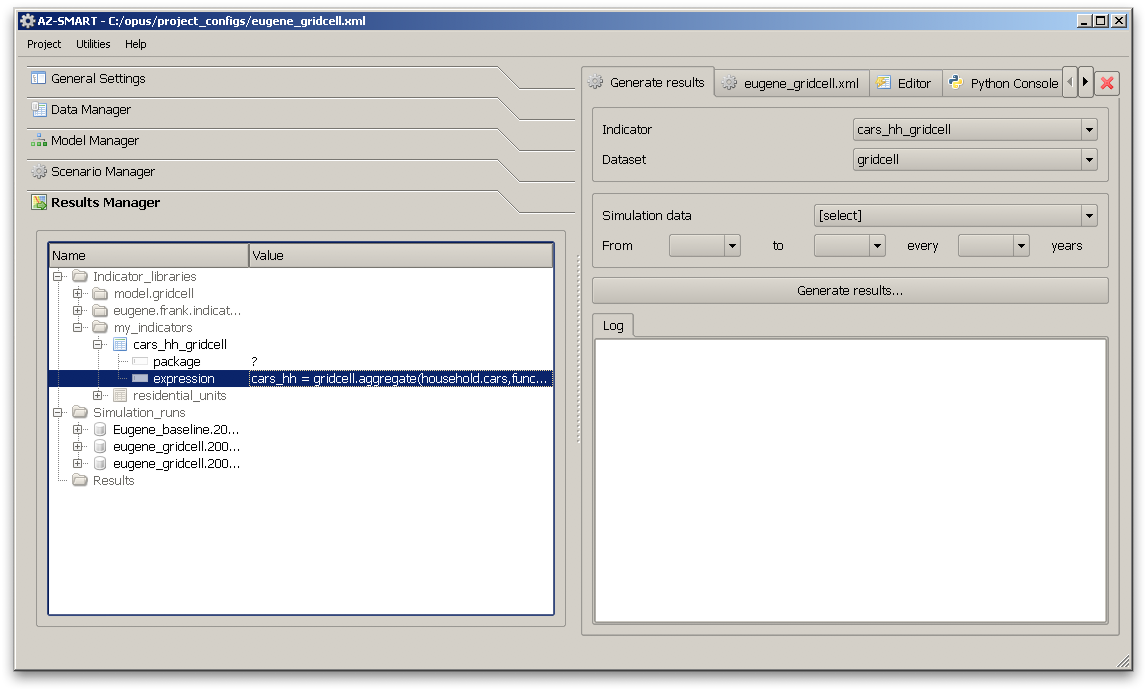
\includegraphics[scale=0.4]{graphics/indicator-cars-gridcell-1.png}
\end{center}
\caption{Generating the Average Cars per Household in a Gridcell}
\label{fig:indicator-cars-gridcell-1}
\end{figure}

\begin{figure}[htp]
\begin{center}
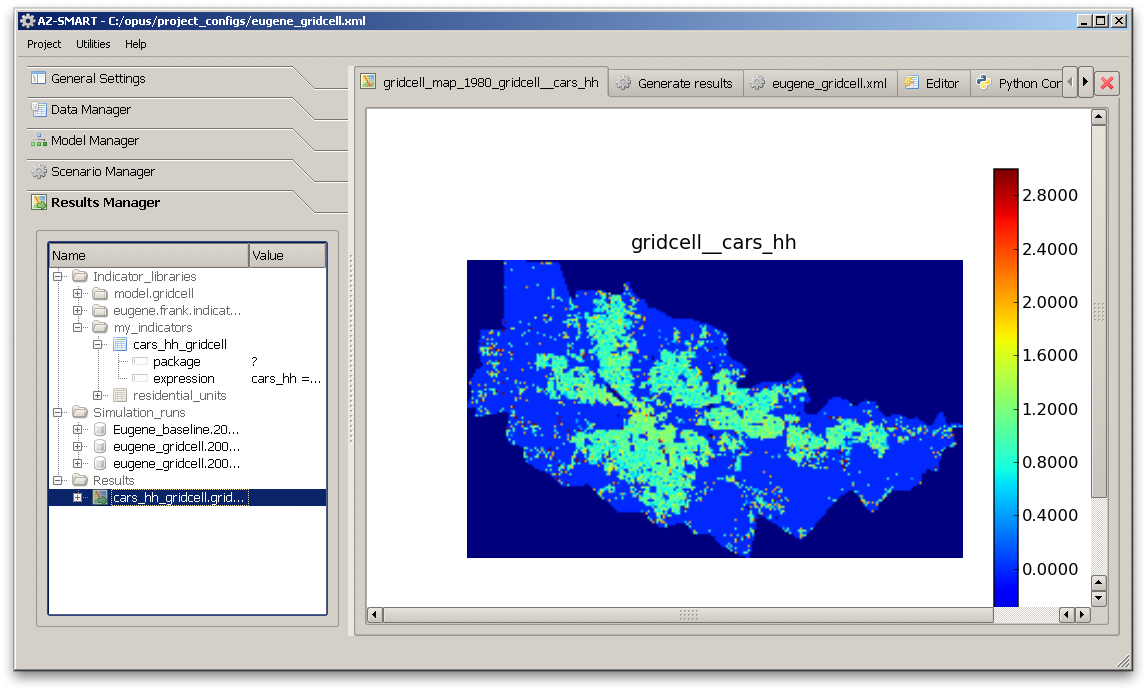
\includegraphics[scale=0.4]{graphics/indicator-cars-gridcell-2.png}
\end{center}
\caption{Generating the Average Cars per Household in a Gridcell}
\label{fig:indicator-cars-gridcell-2}
\end{figure}

In order to compute the second indicator, we will need to average the number of cars per household at the zonal level as follows:

\code{cars\_per\_hh = zone.aggregate(household.cars, intermediates= [gridcell], function=mean)}

The only remaining problem with this is that we cannot display zonal data using Matplotlib, which generates only raster image maps, meaning that it only supports displaying data assigned to gridcells.  Recalling the \verb#disaggregate# function in the expression language, we can just disaggregate the zonal average like this:

\code{cars\_per\_hh = gridcell.disaggregate(zone.aggregate(household.cars, intermediates= [gridcell], function=mean))}

To generate the third indicator of average household size we could use a similar expression:

\code{persons\_per\_hh = zone.aggregate(household.persons, function=mean, intermediates = [gridcell])}

\emph{Unfortunately this zone aggregation will not currently work in the GUI due to some hard coding that assumes indicators added in my\_indicators will be gridcell-based.  This will be fixed shortly.  In the mean time, it would be better to stick to gridcell-based indicators in the my\_indicators section of the Results Manager.}

Now we use a compound expression, to sum the result of two variables, and take the log of the result.  This is to produce the indicator as shown below:

\code{ln\_emp\_pop=ln(urbansim.gridcell.population+urbansim.gridcell.number\_of\_jobs)}

Note that these are variables which can be found on the disk in src/urbansim/gridcell.  The result of visualizing this indicator is shown in Figure \ref{fig:indicator-ln-emp-pop}.

\begin{figure}[htp]
\begin{center}
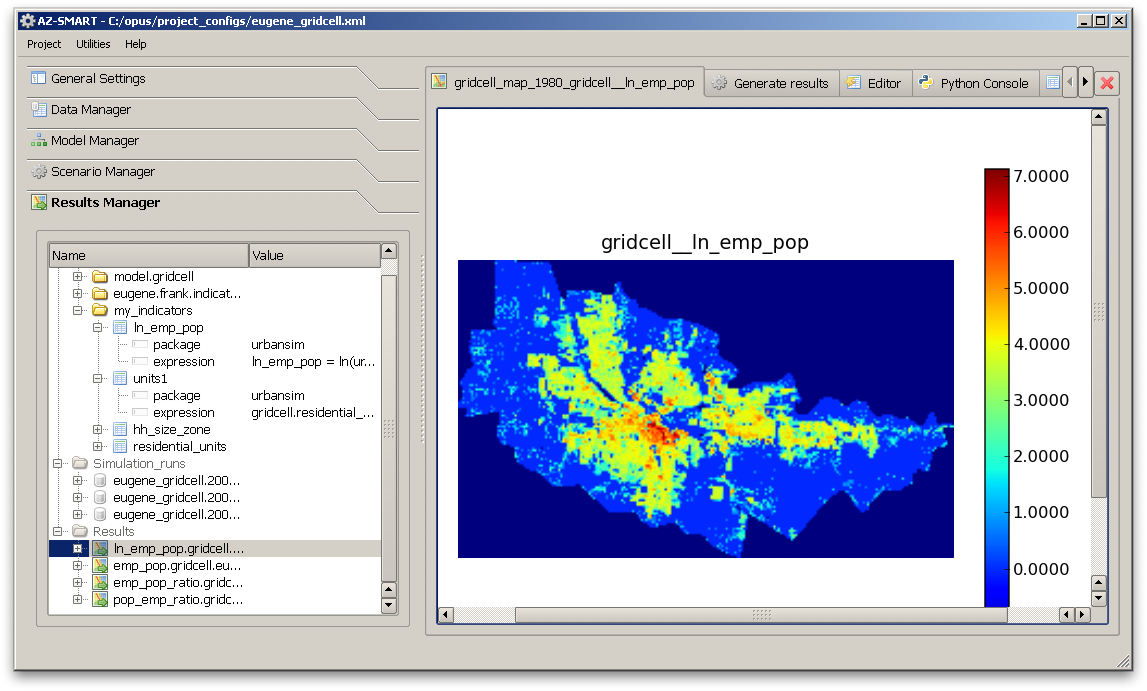
\includegraphics[scale=0.4]{graphics/indicator-ln-emp-pop.png}
\end{center}
\caption{Log of (Population + Employment) by Gridcell}
\label{fig:indicator-ln-emp-pop}
\end{figure}

For the last two indicators in the list to be done, we return to indicators that are already defined in a generic indicator library in the results manager.  To produce the population by zone indicator and visualize it as a table, use the following steps.  Right-click on the population indicators, and select \verb#Generate results with#.  In the form that is created on the right, select the pull-down menu labeled \verb#Dataset# and click on zone.  This is a generalized indicator that uses a simple mechanism to allow different levels of aggregation to be selected in this way, without the need to type in an expression as was done in the preceding examples.  Select a simulation result, and generate the indicator.  Then select the new indicator result containing the indicator values, right-click, and select \verb#View result as# and choose \verb#Table#.  This should generate a browsable table in the form window, as shown below in Figure \ref{fig:indicator-population-zone-table}.

\begin{figure}[htp]
\begin{center}
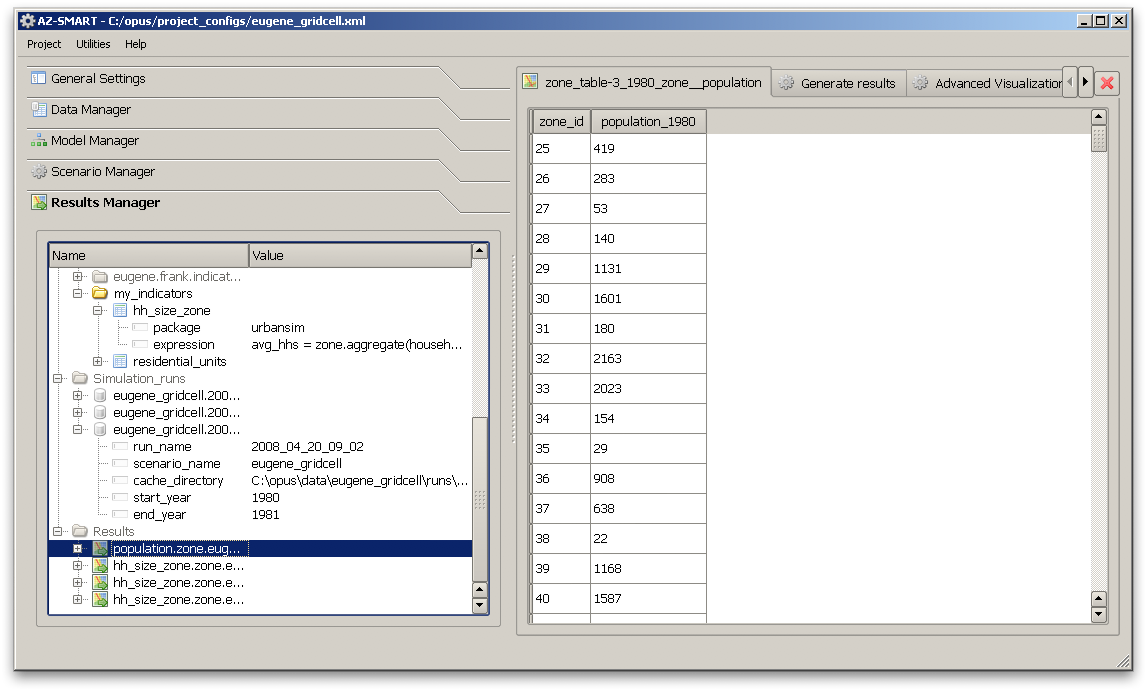
\includegraphics[scale=0.4]{graphics/indicator-population-zone-table.png}
\end{center}
\caption{Viewing the Population by Zone Indicator as a Table}
\label{fig:indicator-population-zone-table}
\end{figure}

Now that we have seen the integrated Matplotlib maps, you might want to know how to export an indicator to a more full-featured GIS system such as ArcGIS (a commercial package from Environmental Systems Research Institute), or PostGIS (an open source package built on the Postgres database).  The Results Manager is now able to export a table with one or more indicators to an ESRI Geodatabase for further analysis and visualization.  In the following example, we export the same indicator result shown above as a table, to an ESRI File-based Geodatabase.  Other Geodatabase formats are also supported.

If the population by zone table result is still available, right-click on the result in the tree on the left-hand side of the window, and select the \verb#View result as# and choose \verb#Advanced visualization#.  It will generate a form as shown in Figure \ref{fig:indicator-population-zone-export}.  We need to add the indicator we have generated to the set, in the upper portion of this form, and select the location of the ESRI geodatabase.  I am assuming that the geodatabase contains a \verb#Feature Class# corresponding to the table being exported. In this example, the table corresponds to the zone feature class.  Once the form is filled in, click on the \verb#Go!# button, to start the export process.  A message will be printed to the log to indicate the completion status of this export process.

\begin{figure}[htp]
\begin{center}
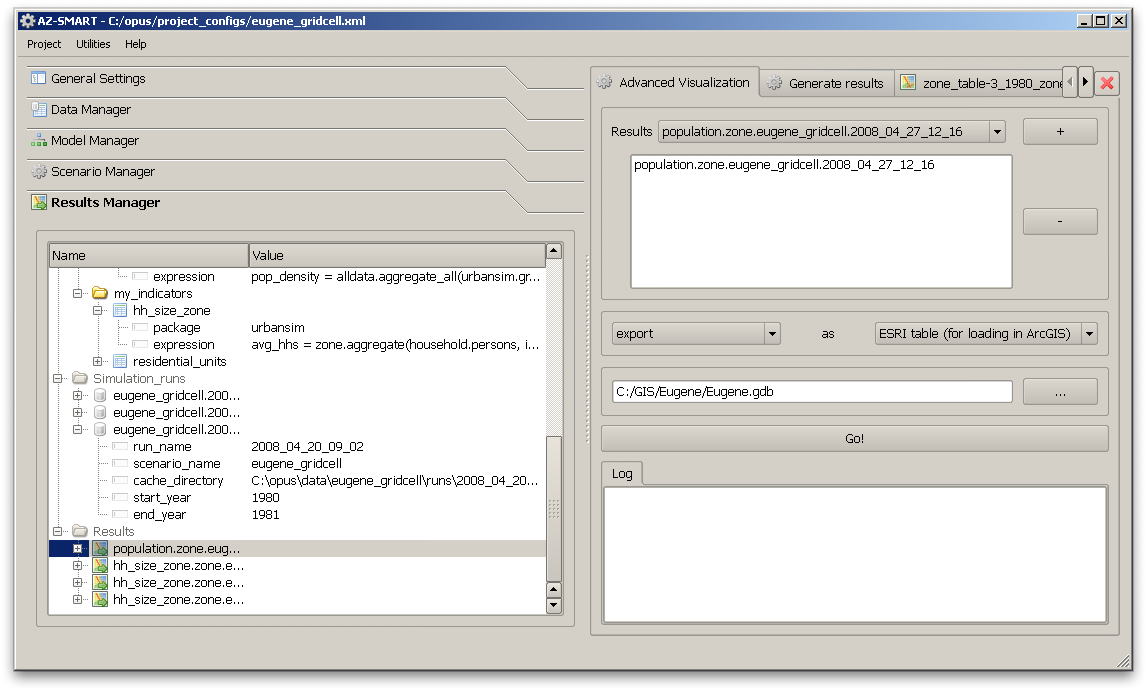
\includegraphics[scale=0.4]{graphics/indicator-population-zone-export.png}
\end{center}
\caption{Exporting the Population by Zone Indicator to an ESRI Geodatabase}
\label{fig:indicator-population-zone-export}
\end{figure}

Once the export is successfully completed, the geodatabase will contain a table that contains the indicator result, with a zone\_id and an ArcGIS \verb#OBJECTID*# that corresponds to the internal object ids in the feature class.  It is safe to join the indicator table result with the feature class using either the objectid or the zone\_id.  The map in Figure \ref{fig:indicator-population-zone-arcgis} shows the result of joining the feature class with the indicator table and generating a thematic map of the populaion by zone, using the zone.acres field to normalize the population, resulting in a map of population density per acre.

\begin{figure}[htp]
\begin{center}
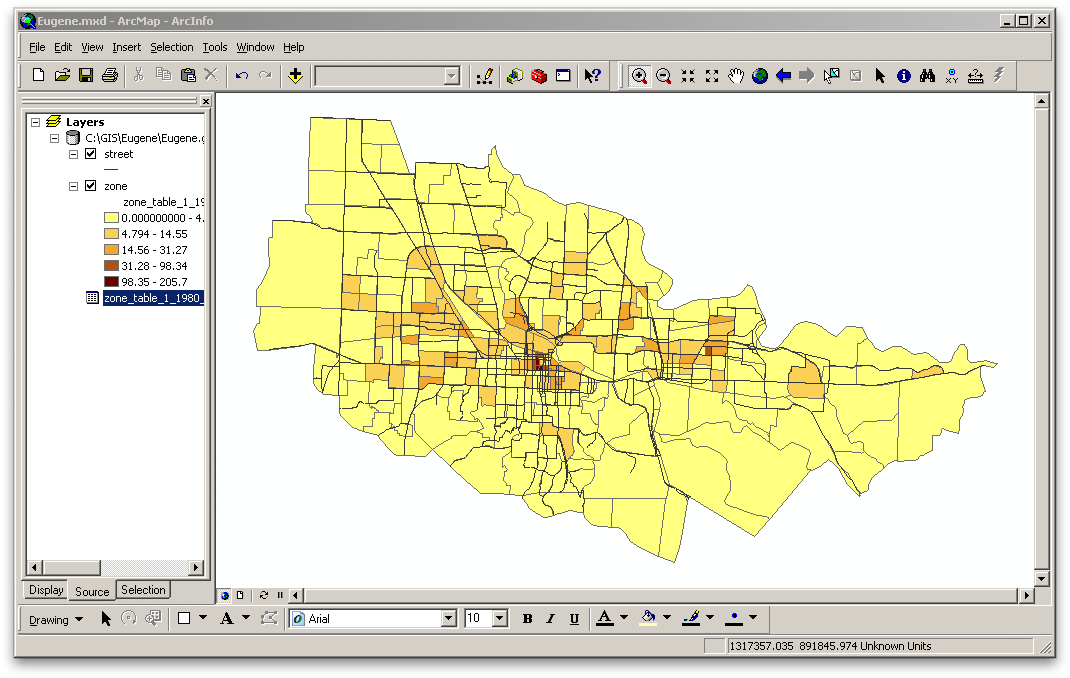
\includegraphics[scale=0.4]{graphics/indicator-population-zone-arcgis.png}
\end{center}
\caption{Mapping the Population by Zone Indicator in ESRI ArcMap}
\label{fig:indicator-population-zone-arcgis}
\end{figure}

